\documentclass[a4paper,11pt]{article}
\usepackage{graphicx,url}
\usepackage[T1]{fontenc}
\usepackage[utf8]{inputenc}
\usepackage[brazil]{babel}
\usepackage{a4wide}
\usepackage{booktabs}
\graphicspath{{./imagens/}}
\title{\vspace{-4cm}Relatório 04 - Laboratório de Arquitetura de Computadores}
\author{Luiz Junio Veloso Dos Santos - Matricula: 624037}

\begin{document} 

\maketitle

\begin{table}[h!]
    \centering
    \begin{tabular}{@{}|r|l|l|l|l|l|l|l|l|@{}}
        \toprule
        S=                                                      & 0000 & 0001 & 0010 & 0011 & 0100 & 0101 & 0110 & 0111 \\ \midrule
        \begin{tabular}[c]{@{}r@{}}A=0000\\ B=0000\end{tabular} & 1111 & 1111 & 0000 & 0000 & 1111 & 1111 & 0000 & 0000 \\ \midrule
        \begin{tabular}[c]{@{}r@{}}A=0001\\ B=0001\end{tabular} & 1110 & 1110 & 0000 & 0000 & 1110 & 1110 & 0000 & 0000 \\ \midrule
        \begin{tabular}[c]{@{}r@{}}A=0010\\ B=0010\end{tabular} & 1101 & 1101 & 0000 & 0000 & 1101 & 1101 & 0000 & 0000 \\ \midrule
        \begin{tabular}[c]{@{}r@{}}A=0100\\ B=0100\end{tabular} & 1011 & 1011 & 0000 & 0000 & 1011 & 1011 & 0000 & 0000 \\ \midrule
        \begin{tabular}[c]{@{}r@{}}A=1000\\ B=1000\end{tabular} & 0111 & 0111 & 0000 & 0000 & 0111 & 0111 & 0000 & 0000 \\ \bottomrule
    \end{tabular}
\end{table}

\begin{table}[h!]
    \centering
    \begin{tabular}{@{}|r|l|l|l|l|l|l|l|l|@{}}
        \toprule
        S=                                                      & 1000 & 1001 & 1010 & 1011 & 1100 & 1101 & 1110 & 1111 \\ \midrule
        \begin{tabular}[c]{@{}r@{}}A=0000\\ B=0000\end{tabular} & 1111 & 1111 & 0000 & 0000 & 1111 & 1111 & 0000 & 0000 \\ \midrule
        \begin{tabular}[c]{@{}r@{}}A=0001\\ B=0001\end{tabular} & 1111 & 1111 & 0001 & 0001 & 1111 & 1110 & 0001 & 0001 \\ \midrule
        \begin{tabular}[c]{@{}r@{}}A=0010\\ B=0010\end{tabular} & 1111 & 1111 & 0010 & 0010 & 1111 & 1101 & 0010 & 0010 \\ \midrule
        \begin{tabular}[c]{@{}r@{}}A=0100\\ B=0100\end{tabular} & 1111 & 1111 & 0100 & 0100 & 1111 & 1011 & 0100 & 0100 \\ \midrule
        \begin{tabular}[c]{@{}r@{}}A=1000\\ B=1000\end{tabular} & 1111 & 1111 & 1000 & 1000 & 1111 & 0111 & 1000 & 1000 \\ \bottomrule
    \end{tabular}
\end{table}
\newpage
\begin{enumerate}
    \item \textbf{Simulador 97:}
        \begin{figure}[h!]
            \caption{Primeira função lógica para A=0 B=0}
            \centering
            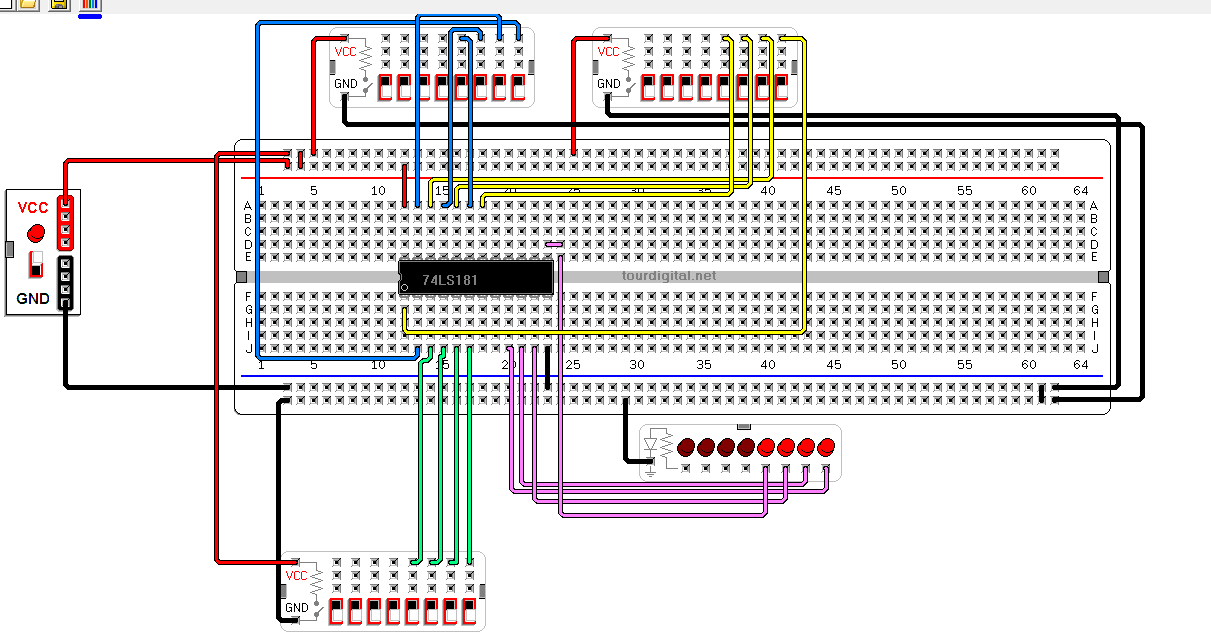
\includegraphics[width=1\textwidth]{simulador0}
        \end{figure}  
        \begin{figure}[h!]
            \caption{Segunda função lógica para A=0 B=0}
            \centering
            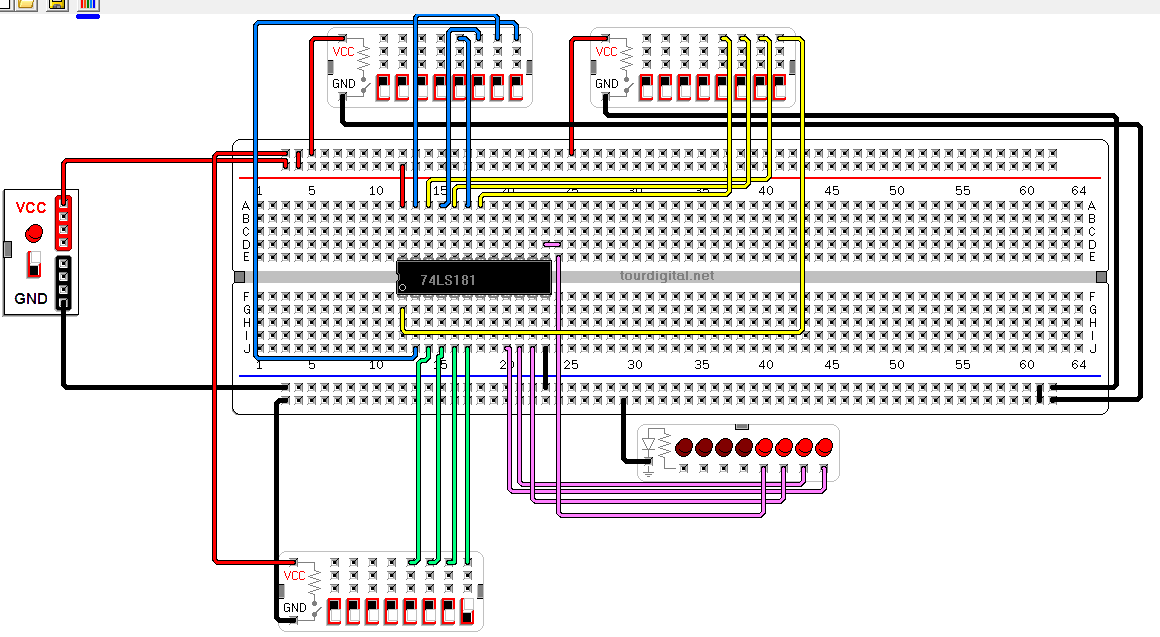
\includegraphics[width=1\textwidth]{simulador1}
        \end{figure}
        \newpage
        \begin{figure}[ht!]
            \caption{Terceira função lógica para A=0 B=0}
            \centering
            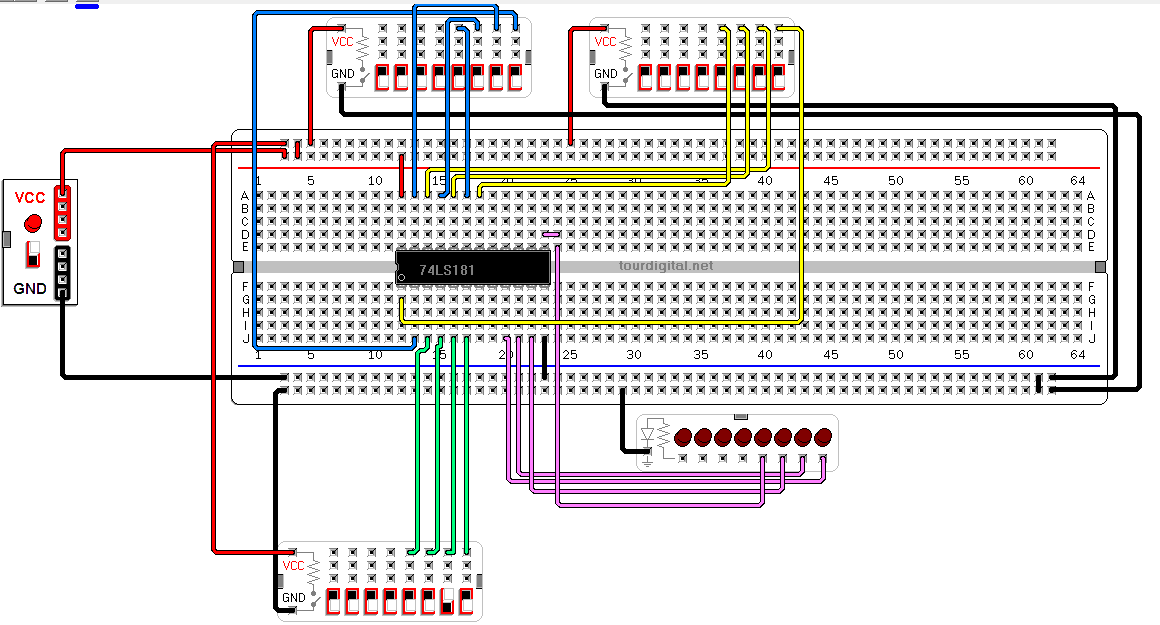
\includegraphics[width=1\textwidth]{simulador2}
        \end{figure} 
    \item \textbf{Logisim:} 
        \begin{figure}[ht!]
            \caption{ULA}
            \centering
            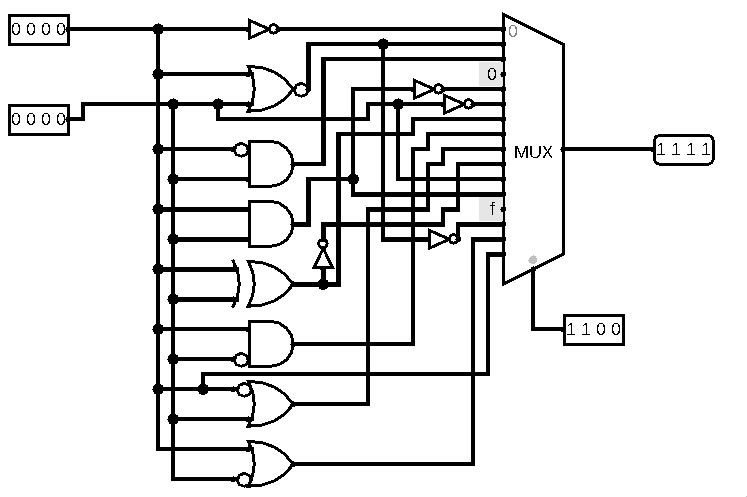
\includegraphics[width=1\textwidth]{logisim-ULA}
        \end{figure}    
\end{enumerate}

\end{document}
